
\chapter{Phân tích kết cấu và lựa chọn cơ cấu chấp hành}

\section{Phân tích kết cấu robot}

\subsection{Thiết kế thân}
Thân của robot bốn chân là bộ phận trung tâm của toàn bộ kết cấu robot. Bốn chân được liên kết với nhau thông qua thân, do đó thiết kế thân cần đáp ứng các yêu cầu sau: 

Thứ nhất, phải có độ bền đủ lớn để đảm bảo không xảy ra biến dạng, nứt gãy,… trong quá trình robot di chuyển. 

Thứ hai, để đạt được khả năng di chuyển linh hoạt và hiệu quả năng lượng cao, thân robot cần được thiết kế nhẹ nhất có thể. 

Ngoài ra, bên trong thân robot phải có không gian đủ lớn để lắp đặt các servo, pin, bo mạch điều khiển, module chuyển đổi điện áp và các linh kiện khác. 

Cuối cùng, 12 servo được lắp tại các khớp chân cần có thiết kế riêng cho đường đi dây và vị trí lắp đặt, vì chúng luôn chuyển động tương đối so với thân robot khi robot đi bộ hoặc chạy chậm. 

Dựa trên các yêu cầu trên, thân robot được thiết kế theo dạng liền khối, nhằm ngăn ngừa biến dạng hoặc gãy vỡ. 

Bốn góc của thân được thiết kế để kết nối với cụm khớp hông, đảm bảo không xảy ra giao thoa cơ khí khi khớp hông quay theo bất kỳ hướng nào. 

Ngoài ra, tại những vị trí có khả năng chịu tải thấp, cấu trúc được khoét rỗng hợp lý để giảm khối lượng. Mô hình 3D của cấu trúc thân robot bốn chân được thể hiện ở Hình \ref{fig12-c} bên dưới.

\begin{figure}[H]
    \centering
    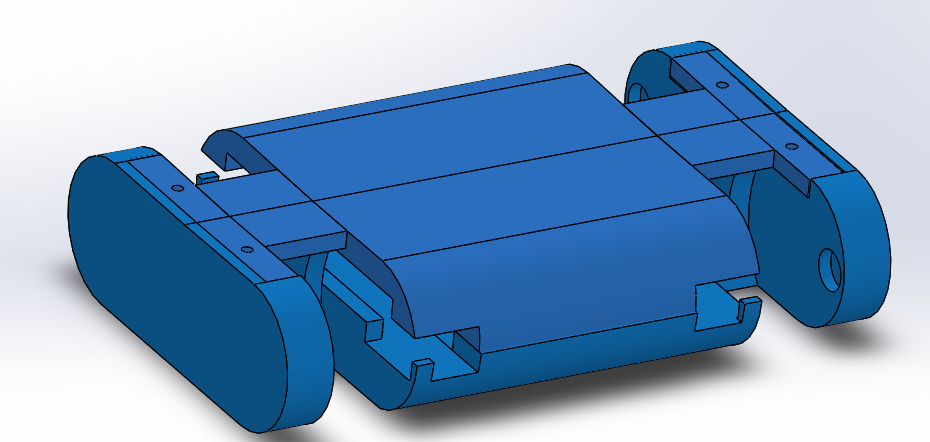
\includegraphics[width=0.6\textwidth]{img/fig12-c-body.png}
    \caption{Thiết kế thân liền khối nhằm đạt độ bền cao và khối lượng nhẹ.}
    \label{fig12-c}
\end{figure}

\begin{figure}[H]
    \centering
    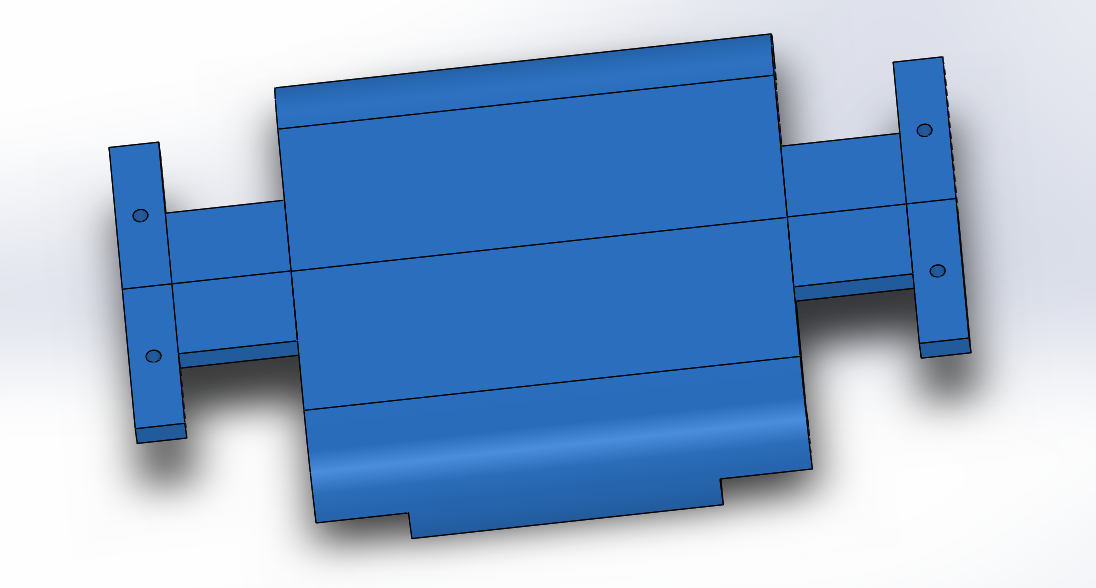
\includegraphics[width=0.6\textwidth]{img/fig12-b-nắp thân.png}
    \caption{Nắp thân.}
    \label{fig12-b}
\end{figure}

\begin{figure}[H]
    \centering
    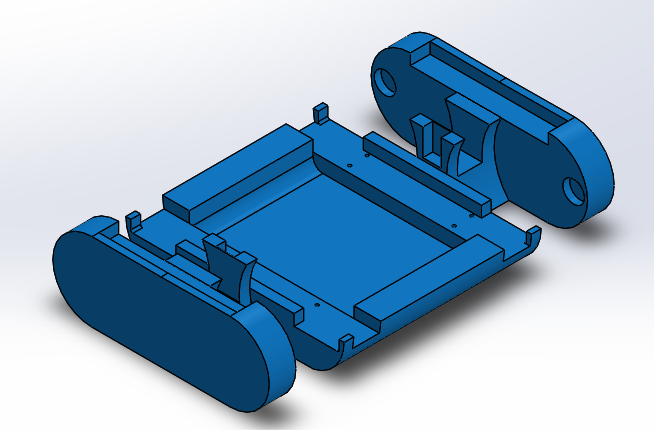
\includegraphics[width=0.6\textwidth]{img/fig12-a-thân.png}
    \caption{Thiết kế thân.}
    \label{fig12-a}
\end{figure}


\subsection{Thiết kế khớp hông}

Khớp hông của robot bốn chân được thiết kế để tạo ra hai bậc tự do, một cho chuyển động roll và một cho chuyển động pitch. Mỗi chuyển động được truyền động bởi một servo.

Do servo được sử dụng trong thiết kế của chúng tôi là loại servo một trục, các ổ bi mặt bích 626zz được sử dụng ở phía đối diện trục servo nhằm giảm lực hướng kính tác dụng lên trục. Đầu trục và khớp hông được tích hợp trong quá trình chế tạo, điều này giúp thuận tiện cho việc lắp đặt và giảm sai số lắp ráp.

Ngoài ra, servo điều khiển chuyển động vung trước (tức là chuyển động pitch) của khớp hông được lắp bên trong giá đỡ khớp hông để tiết kiệm không gian. Mô hình 3D của cụm khớp hông được thể hiện trong Hình \ref{fig13}.

\begin{figure}[H]
    \centering
    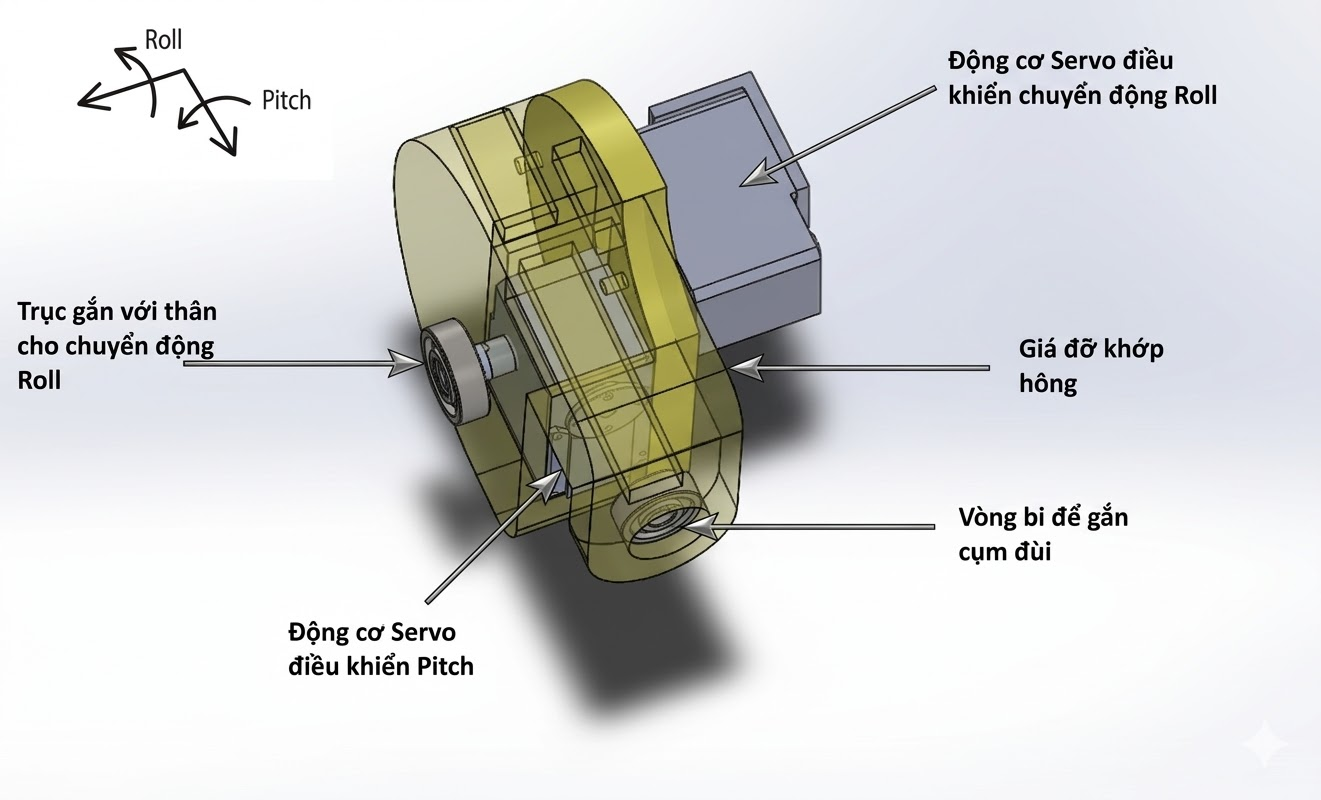
\includegraphics[width=0.6\textwidth]{img/fig13-Hip-joint assembly for the lateral and longitudinal swing motions..jpg }
    \caption{Cụm khớp hông cho chuyển động vung ngang và vung dọc.}
    \label{fig13}
\end{figure}

\subsection{Thiết kế chân}

Chân của robot bốn chân thường xuyên tiếp xúc với mặt đất để tạo lực đẩy, do đó thiết kế chân đóng vai trò quan trọng đối với khả năng di chuyển thành công của robot.

Chuyển động vung trước của khớp hông (phần đùi) sử dụng ổ bi để chịu lực dọc trục. Vì khối lượng của chân đã được bỏ qua trong các tính toán động học trình bày bên dưới, nên phần đùi và cẳng chân cần được thiết kế sao cho khối lượng và mô men quán tính nhỏ nhất có thể nhằm giảm sai số lý thuyết.

Trong thiết kế này, thay vì sử dụng kết nối servo trực tiếp tại khớp gối, một cơ cấu liên kết đầu bi (ball-head linkage) được sử dụng, trong đó cẳng chân được truyền động gián tiếp thông qua tay đòn (rocker arm) của servo. Cách bố trí này cho phép đặt servo ở phía trên của đùi, gần khớp hông, nơi mô men quán tính quay của chân tương đối nhỏ.

Mô hình lắp ráp một chân đơn được thể hiện trong Hình \ref{fig14}.

\begin{figure}[H]
    \centering
    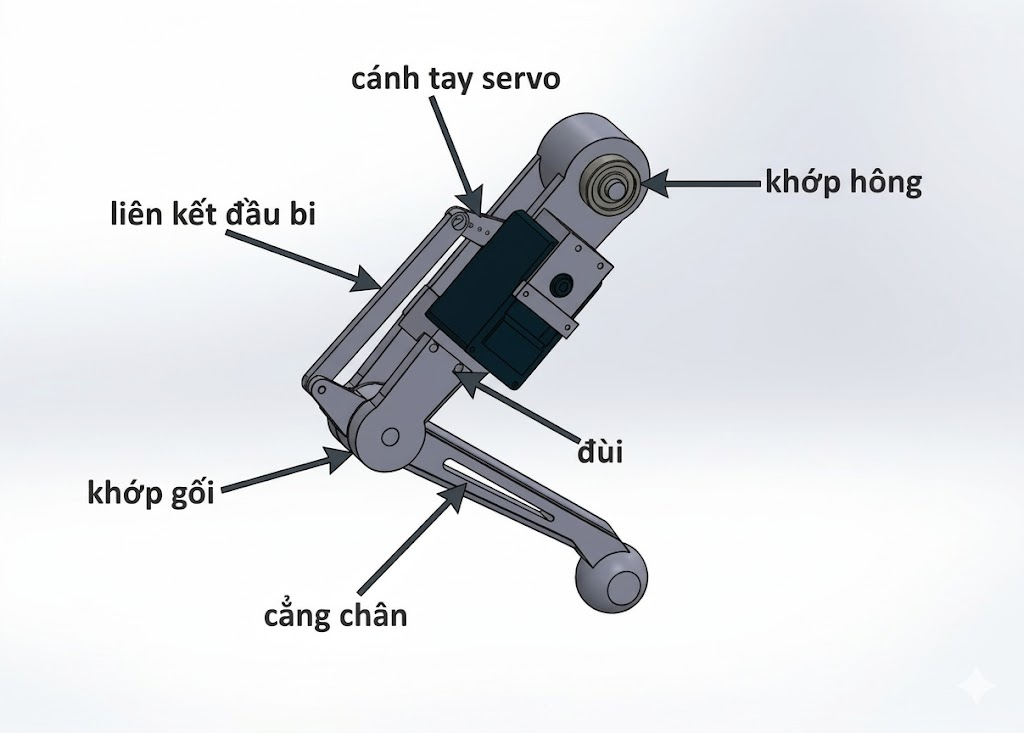
\includegraphics[width=0.6\textwidth]{img/fig14- Single leg assembly..jpg}
    \caption{Cụm lắp ráp một chân đơn.}
    \label{fig14}
\end{figure}

Dựa trên cấu trúc chân của robot bốn chân, có thể thấy rằng cẳng chân là bộ phận dễ bị gãy và uốn cong nhất vì nó phải chịu trọng lượng của toàn bộ robot cũng như các lực nén khi tiếp xúc với mặt đất. 

Ở đây, lực tiếp xúc với mặt đất được đơn giản hóa chỉ gồm lực pháp tuyến $F_N$ và lực tiếp tuyến $F_\mu$ trong mặt phẳng thẳng đứng, như thể hiện ở Hình \ref{fig15}.

Khi cẳng chân quay quanh trục khớp gối, nếu bỏ qua ma sát tại khớp và ma sát tiếp xúc với mặt đất, mô-men tải ngoài lớn nhất có thể được xác định theo công thức:

\begin{equation}
    T_{\text{max}} = \eta F_N L_3 \sin(\alpha)
\end{equation}

trong đó $F_N$ là lực pháp tuyến, $L_3$ là khoảng cách từ trục khớp gối đến điểm tiếp xúc mặt đất, $\alpha$ là góc giữa cẳng chân và phương thẳng đứng và $\eta$ là hệ số tải động.

Bằng cách định nghĩa các thuộc tính vật liệu phù hợp cho từng bộ phận của robot bốn chân trong mô hình SolidWorks, tổng khối lượng robot thu được xấp xỉ $M = 2.3\text{ kg}$.

Giả sử bốn chân chịu đều toàn bộ trọng lượng của robot trong trạng thái tĩnh, lực pháp tuyến được tính là:

\begin{equation}
    F_N = \frac{Mg}{4}
\end{equation}

Trong phân tích bền số học dưới đây, sử dụng các giá trị: chiều dài cẳng chân $L_3 = 0.125\text{ m}$, góc nghiêng $\alpha = 45^\circ$, và hệ số tải động $\eta = 1.2$.

\section{Phân tích vật liệu và công nghệ chế tạo}

\subsection{Lựa chọn vật liệu in 3D}

Toàn bộ các chi tiết cơ khí của robot (thân, giá đỡ khớp hông, đùi, cẳng chân) được chế tạo bằng công nghệ in 3D FDM (Fused Deposition Modeling). Vật liệu được lựa chọn là PLA (Polylactic Acid) --- một loại nhựa sinh học phổ biến trong prototyping nhanh. Bảng~\ref{tab:pla_props} trình bày các thuộc tính cơ học chính của PLA so với một số vật liệu thay thế.

\begin{table}[H]
\centering
\caption{So sánh thuộc tính cơ học các vật liệu in 3D phổ biến}
\label{tab:pla_props}
\renewcommand{\arraystretch}{1.3}
\begin{tabular}{|l|c|c|c|c|}
\hline
\textbf{Thuộc tính} & \textbf{PLA} & \textbf{ABS} & \textbf{PETG} & \textbf{Nylon} \\ \hline
Giới hạn bền kéo (MPa) & 50--60 & 35--45 & 50--55 & 70--85 \\ \hline
Mô đun đàn hồi (GPa) & 3,5 & 2,1 & 2,0 & 1,5--2,5 \\ \hline
Tỷ trọng (g/cm$^3$) & 1,24 & 1,04 & 1,27 & 1,14 \\ \hline
Nhiệt độ biến dạng ($^\circ$C) & 56 & 98 & 72 & 180 \\ \hline
Độ khó in & Thấp & Trung bình & Trung bình & Cao \\ \hline
Giá thành & Thấp & Trung bình & Trung bình & Cao \\ \hline
\end{tabular}
\end{table}

PLA được chọn vì các lý do sau:
\begin{itemize}
    \item \textbf{Độ cứng cao:} Mô đun đàn hồi $E = 3{,}5$ GPa là cao nhất trong các vật liệu in 3D phổ biến, giúp giảm biến dạng dưới tải trọng.
    \item \textbf{Dễ in:} Nhiệt độ đùn thấp ($200$--$210^\circ$C), không cần bàn sấy nóng, ít cong vênh (warping).
    \item \textbf{Chi phí thấp:} Phù hợp với giai đoạn prototyping và nghiên cứu.
    \item \textbf{Bề mặt mịn:} Chất lượng bề mặt tốt, giảm ma sát tại các vùng tiếp xúc khớp.
\end{itemize}

Tuy nhiên, PLA có nhược điểm là giòn (dễ gãy khi va đập mạnh) và chịu nhiệt kém (biến dạng trên $56^\circ$C). Để khắc phục, các vùng chịu lực tập trung (như đầu nối khớp hông) được in với mật độ điền (infill density) 80--100\%, cao hơn so với mức 30--40\% thông thường.

\subsection{Tham số in 3D}

Bảng~\ref{tab:print_params} trình bày các tham số in 3D được sử dụng để chế tạo các chi tiết cơ khí.

\begin{table}[H]
\centering
\caption{Tham số in 3D cho các chi tiết robot}
\label{tab:print_params}
\renewcommand{\arraystretch}{1.3}
\begin{tabular}{|l|c|l|}
\hline
\textbf{Tham số} & \textbf{Giá trị} & \textbf{Ghi chú} \\ \hline
Chiều cao lớp in (layer height) & 0,2 mm & Cân bằng tốc độ và chất lượng \\ \hline
Số vỏ ngoài (wall count) & 4 & Tăng độ bền \\ \hline
Mật độ điền -- thân & 40\% & Pattern: gyroid \\ \hline
Mật độ điền -- khớp & 80--100\% & Chịu lực tập trung \\ \hline
Nhiệt độ đùn & 210$^\circ$C & PLA+ \\ \hline
Tốc độ in & 50 mm/s & Đảm bảo bám dính lớp \\ \hline
Hỗ trợ (support) & Có & Cho các góc nhô > 45$^\circ$ \\ \hline
\end{tabular}
\end{table}

Tổng thời gian in cho toàn bộ chi tiết robot (thân, nắp thân, 4 bộ khớp hông, 4 đùi, 4 cẳng chân, phụ kiện) là khoảng 35--40 giờ. Sau khi in, các chi tiết được xử lý hậu kỳ: loại bỏ support, chà nhám bề mặt tiếp xúc khớp, và khoan lỗ cho ốc vít M3 cùng ổ bi 626zz.

\subsection{Phân tích tải trọng bằng SolidWorks Simulation}

Để kiểm chứng độ bền của thiết kế, nhóm đã thực hiện phân tích phần tử hữu hạn (FEA -- Finite Element Analysis) trên phần mềm SolidWorks Simulation cho chi tiết cẳng chân --- bộ phận chịu tải lớn nhất. Các điều kiện biên được đặt là:

\begin{itemize}
    \item \textbf{Ràng buộc:} Cố định đầu trên cẳng chân (vùng nối với khớp gối).
    \item \textbf{Tải trọng:} Lực pháp tuyến $F_N = 11{,}28$ N tại đầu dưới cẳng chân (bàn chân), hướng dọc theo trục chân.
    \item \textbf{Vật liệu:} PLA với $E = 3{,}5$ GPa, $\sigma_{yield} = 50$ MPa.
\end{itemize}

Kết quả phân tích cho thấy ứng suất Von Mises cực đại trên cẳng chân đạt khoảng $12$ MPa, nhỏ hơn nhiều so với giới hạn chảy $50$ MPa của PLA, cho hệ số an toàn $n = 50/12 \approx 4{,}2$. Giá trị này xác nhận thiết kế cẳng chân đủ bền cho vận hành bình thường.

\section{Lựa chọn cơ cấu chấp hành}
Việc lựa chọn cơ cấu chấp hành có ảnh hưởng lớn đến hiệu năng di chuyển của robot bốn chân. Do trọng lượng bản thân của robot, cơ cấu chấp hành cần tạo ra mô-men xoắn lớn, đáp ứng nhanh và có kích thước nhỏ gọn.

Động cơ không chổi than được sử dụng rộng rãi nhờ đặc tính động học vượt trội, tuy nhiên chúng thường có giá thành cao và kích thước lớn.

Vì trọng tâm chính của đồ án này là triển khai và đánh giá sơ bộ thuật toán dáng đi trên mô hình robot kích thước để bàn, nên servo được lựa chọn làm nguồn truyền động.

Được trang bị khả năng phản hồi góc quay trực tiếp theo thời gian thực cùng tỷ số truyền bánh răng lớn, loại servo này cho phép vi điều khiển dễ dàng thực hiện điều khiển vòng kín. Điều này là nền tảng thiết yếu để chạy các node tính toán động học nghịch, giúp robot tự bù trừ sai số trong các thử nghiệm dáng đi phức tạp và tự cân bằng chính xác hơn.

Mẫu servo được sử dụng là ST3215 và ST3215-HS, như thể hiện ở Hình \ref{fig16}, và các thông số kỹ thuật cụ thể được trình bày trong Bảng \ref{tab:1}.

\begin{figure}[H]
    \centering
    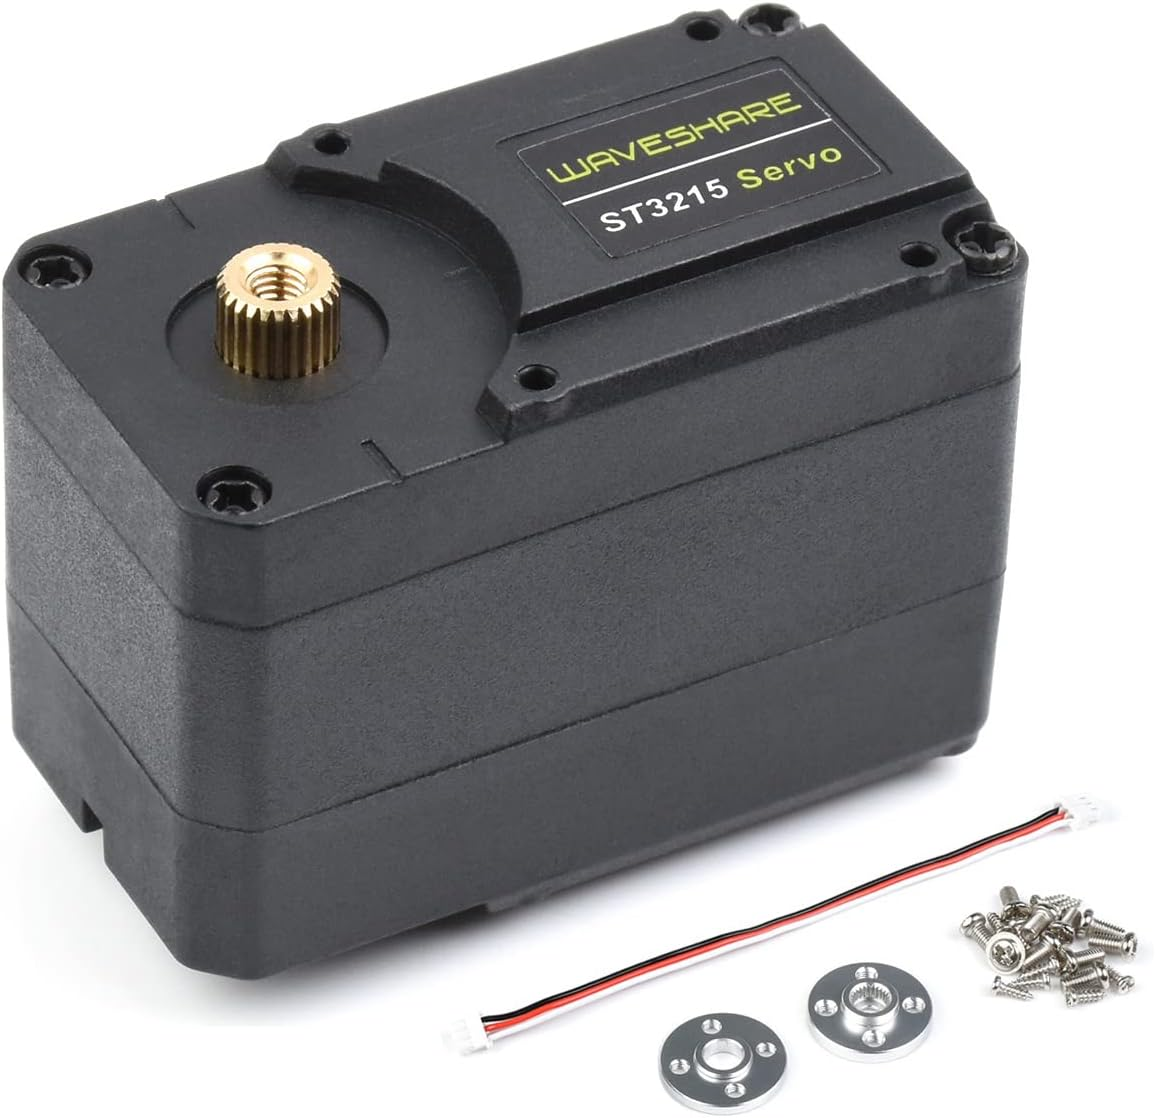
\includegraphics[width=0.6\textwidth]{img/fig16-ST3215.jpg}
    \caption{Cơ cấu chấp hành servo ST3215 dùng cho robot bốn chân.}
    \label{fig16}
\end{figure}

\begin{table}[htbp]
    \centering
    \caption{Thông số kỹ thuật của động cơ servo ST3215 và ST3215-HS.}
    \label{tab:1}
    \resizebox{\textwidth}{!}{% Thu nhỏ bảng vừa với chiều rộng trang giấy
        \begin{tabular}{l c c c c c c c}
            \toprule
            \textbf{Mẫu} & \textbf{Trọng lượng} & \textbf{\makecell{Kích thước \\ (L $\times$ W $\times$ H)}} & \textbf{\makecell{Điện áp \\ hoạt động}} & \textbf{\makecell{Tốc độ truyền \\ (Baudrate)}} & \textbf{\makecell{Phạm vi \\ góc quay}} & \textbf{Tốc độ tối đa} & \textbf{Lực xoắn tối đa} \\
            \midrule
            ST3215 & 69 g & \makecell{$45.2 \times 24.7 \times$ \\ $35.0$ mm} & 6.0 V -- 12.6 V & \textasciitilde 1 Mbps & \makecell{360$^\circ$ } & 0.222 s/60$^\circ$ (@12 V) & 30 kg$\cdot$cm (@12 V) \\
            \addlinespace % Thêm một khoảng trắng nhỏ giữa 2 hàng cho thoáng
            ST3215-HS & 68 g & \makecell{$45.2 \times 24.7 \times$ \\ $35.0$ mm} & 6.0 V -- 12.6 V & \textasciitilde 1 Mbps & \makecell{360$^\circ$ } & 0.094 s/60$^\circ$ (@12 V) & 20 kg$\cdot$cm (@12 V) \\
            \bottomrule
        \end{tabular}
    }
\end{table}

Để kiểm chứng mô-men xoắn định mức của servo đã chọn, tiến hành phân tích như sau. Dựa trên phân tích ở Mục 3.1.3, ảnh hưởng của mô-men xoắn lên cẳng chân là đáng kể nhất. Gọi góc giữa lực pháp tuyến tiếp xúc mặt đất $F_N$ và cẳng chân $L_3$ là $\alpha$. Như thể hiện trong Hình \ref{fig17}, mô-men do lực tiếp đất tác dụng lên khớp gối là:
\begin{equation}
    M_{\text{knee}} = \eta F_N L_3 \sin(\alpha)
\end{equation}
Mô-men này được cân bằng bởi lực truyền $F_t$ dọc theo thanh liên kết $CD$:
\begin{equation}
    M_{\text{knee}} = F_t L_{CB} \sin(\gamma)
\end{equation}
với $\gamma$ là góc giữa thanh liên kết $CD$ và cánh tay đòn $CB$. Mô-men tác dụng lên trục servo (qua cánh tay đòn $DE$) là:
\begin{equation}
    T_{\text{knee}} = F_t L_{DE} \sin(\beta)
\end{equation}
với $\beta$ là góc giữa thanh $CD$ và tay đòn $DE$. Trong thiết kế cơ cấu gần với hình bình hành, $\gamma \approx \beta$, do đó tỉ số $\sin(\beta)/\sin(\gamma) \approx 1$. Từ đó ta suy ra mô-men yêu cầu tại servo cẳng chân là:
\begin{equation}
    T_{\text{knee}} \approx \eta F_N L_3 \sin(\alpha) \frac{L_{DE}}{L_{CB}}
\end{equation}
Trong dáng đi trot, luôn có hai chân tiếp xúc mặt đất, do đó tải trọng lớn nhất tác dụng lên một chân là:
\begin{equation}
    F_N = \frac{Mg}{2}
\end{equation}
Thay các giá trị từ Bảng \ref{tab:2} với $M = 2.3\,\text{kg}$, $L_3 = 0.125\,\text{m}$, $L_{DE} = 0.024\,\text{m}$, $L_{CB} = 0.025\,\text{m}$, hệ số tải động $\eta = 1.2$, góc nghiêng $\alpha = 45^\circ$, và $g = 9.81\,\text{m/s}^2$ vào công thức, ta có $F_N = 11.28\,\text{N}$ và:
\begin{equation}
    T_{\text{knee}} \approx 1.2 \times 11.28 \times 0.125 \times \sin(45^\circ) \times \frac{0.024}{0.025} \approx 1.149\,\text{N}\cdot\text{m} \approx 11.7\,\text{kg}\cdot\text{cm}
\end{equation}

Giá trị này nhỏ hơn mô-men định mức $20\,\text{kg}\cdot\text{cm}$ của servo ST3215-HS, đảm bảo động cơ hoạt động an toàn.

\begin{figure}[H]
    \centering
    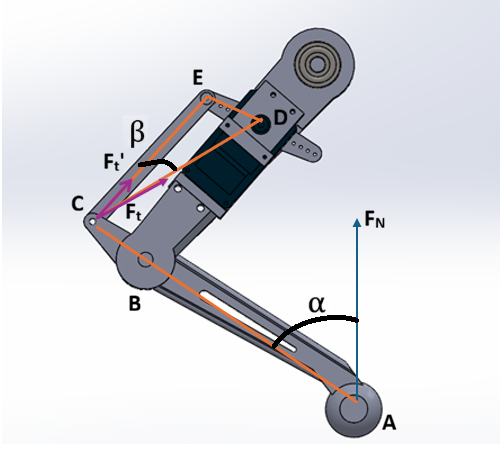
\includegraphics[width=0.6\textwidth]{img/fig17-Torque analysis of the lower leg servo actuator.png}
    \caption{Phân tích mô-men xoắn của cơ cấu chấp hành servo tại cẳng chân.}
    \label{fig17}
\end{figure}

\subsection{Phân tích mô-men khớp vai (Hip Roll)}

Trong thực tế vận hành, để duy trì khả năng thăng bằng và giảm chấn, chân robot không bao giờ duỗi thẳng hoàn toàn. Thay vào đó, phần đùi ($L_2$) và cẳng chân ($L_3$) luôn tạo với nhau một góc gập nhất định như thể hiện ở Hình \ref{fig18}. Việc tính toán mô-men xoắn cần sử dụng khoảng cách thực tế từ khớp hông đến bàn chân. 

Gọi $L_{hd}$ là khoảng cách hiệu dụng từ trục khớp hông đến điểm tiếp xúc mặt đất của bàn chân. Dựa trên định lý hàm số cosin cho tam giác tạo bởi đùi, cẳng chân và góc gập gối $\beta$, ta có:
\begin{equation}
    L_{hd} = \sqrt{L_2^2 + L_3^2 - 2L_2L_3\cos(\beta)}
\end{equation}

Dựa theo Bảng \ref{tab:2} với thiết kế $L_2 = 0.106\,\text{m}$ và $L_3 = 0.125\,\text{m}$, giả sử ở tư thế đi bộ trot tiêu chuẩn robot duy trì góc khuỵu gối $\beta = 90^\circ$ nhằm tối ưu lực bám. Chiều dài hiệu dụng lúc này là:
\begin{equation}
    L_{hd} = \sqrt{0.106^2 + 0.125^2 - 2(0.106)(0.125)\cos(90^\circ)} \approx 0.164\,\text{m}
\end{equation}

Tương tự phân tích trước, tải trọng lớn nhất tác dụng lên một chân là $F_N = 11.28\,\text{N}$, hệ số tải động $\eta = 1.2$, dẫn đến lực tác dụng tổng cộng là $\eta F_N = 13.54\,\text{N}$. 

Công thức tính mô-men xoắn cực đại cho khớp vai $T_{roll}$ theo góc dang chân $\theta_1$ được xác định dựa trên khoảng lệch ngàm $L_1$ và hình chiếu ngang của chiều dài chân hiệu dụng:
\begin{equation}
    T_{roll} = \eta F_N \big(L_1 \cos(\theta_1) + L_{hd} \sin(\theta_1)\big)
\end{equation}

Thay các thông số thiết kế ($L_1 = 0.026\,\text{m}$) vào phương trình, ta thu được:
\begin{equation}
    T_{roll} = 13.54 \times \big(0.026 \cos(\theta_1) + 0.164 \sin(\theta_1)\big) \quad \text{(N}\cdot\text{m)}
\end{equation}

\begin{itemize}
    \item Khi $\theta_1 = 0^\circ$, mô-men tác dụng lên khớp vai chỉ xuất phát từ khoảng lệch ngàm cơ khí: $T_{roll} = 13.54 \times 0.026 \approx 0.35\,\text{N}\cdot\text{m} \approx 3.6\,\text{kg}\cdot\text{cm}$.
    \item Khi $\theta_1 = 15^\circ$, mô-men tăng lên: $T_{roll} \approx 0.91\,\text{N}\cdot\text{m} \approx 9.3\,\text{kg}\cdot\text{cm}$, phản ánh trạng thái robot điều chỉnh tư thế rẽ với góc dang trung bình.
    \item Khi $\theta_1 = 30^\circ$, mô-men đạt giá trị lớn nhất: $T_{roll} \approx 1.41\,\text{N}\cdot\text{m} \approx 14.4\,\text{kg}\cdot\text{cm}$, tương ứng với tình huống bất lợi khi chân dang rộng.
\end{itemize}

Giá trị mô-men cực đại vẫn nhỏ hơn định mức $20\,\text{kg}\cdot\text{cm}$ của servo ST3215-HS, do đó khớp vai vẫn hoạt động trong vùng an toàn, không gây quá tải.

\begin{figure}[H]
    \centering
    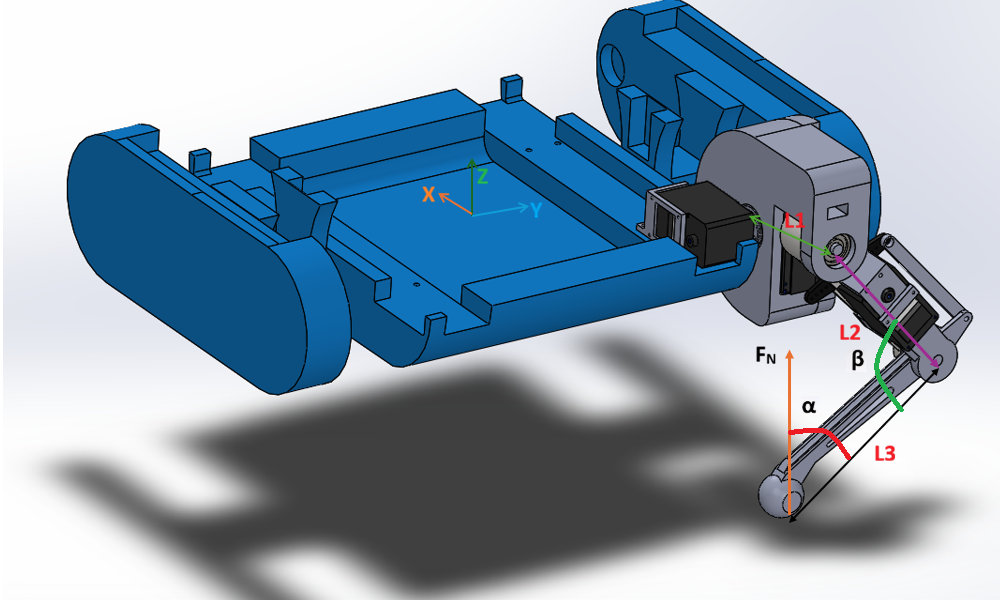
\includegraphics[width=0.6\textwidth]{img/fig18-Free body diagram.png}
    \caption{Mô hình một chân của robot bốn chân.}
    \label{fig18}
\end{figure}

\subsection{Phân tích mô-men khớp hông (Hip Pitch)}

Tương tự quy trình đánh giá ở khớp vai, mô-men xoắn yêu cầu cực đại đối với khớp hông (Pitch) được xác định thông qua chiều dài sải bước hiệu dụng của robot. Trong mặt phẳng dọc, cánh tay đòn tạo ra mô-men phụ thuộc vào độ vươn xa của bàn chân theo phương ngang. Gọi $\alpha$ là góc nghiêng của chân (đường nối từ trục khớp hông đến bàn chân) so với phương thẳng đứng. Phương trình tổng quát tính mô-men xoắn cho khớp hông là:
\begin{equation}
    T_{pitch} = \eta F_N L_{hd} \sin(\alpha)
\end{equation}

Sử dụng khoảng cách hiệu dụng $L_{hd} = 0.164\,\text{m}$ và lực tải $\eta F_N = 13.54\,\text{N}$ đã xác định:
\begin{equation}
    T_{pitch} = 13.54 \times 0.164 \sin(\alpha) = 2.221 \sin(\alpha) \quad \text{(N}\cdot\text{m)}
\end{equation}

Phân tích quỹ đạo chuyển động cho thấy:
\begin{itemize}
    \item Tại tư thế đứng thẳng chân ($\alpha = 0^\circ$), trọng lượng truyền dọc theo chân nên khớp hông không chịu tải uốn ($T_{pitch} = 0$).
    \item Khi chân bước với góc $\alpha = 15^\circ$, mô-men tại khớp hông đạt $T_{pitch} = 2.221 \sin(15^\circ) \approx 0.57\,\text{N}\cdot\text{m} \approx 5.9\,\text{kg}\cdot\text{cm}$. Đây là vùng tải nhẹ, thuận lợi cho động cơ.
    \item Khi $\alpha = 45^\circ$, mô-men tăng lên $T_{pitch} = 2.221 \sin(45^\circ) \approx 1.57\,\text{N}\cdot\text{m} \approx 16.0\,\text{kg}\cdot\text{cm}$, tương ứng với trạng thái vươn dài chân để leo dốc hoặc vượt chướng ngại vật.
\end{itemize}

Giá trị cực đại này vẫn nhỏ hơn đáng kể so với giới hạn mô-men của servo ST3215-HS, xác nhận rằng việc lựa chọn động cơ cho khớp hông là hoàn toàn phù hợp và đảm bảo độ tin cậy trong vận hành.

\subsection{Thiết kế tổng thể}

Thiết kế tổng thể của robot bốn chân được thể hiện trong Hình \ref{fig19}, với tổng cộng 12 bậc tự do và cấu hình chân full-elbow. Ở đây, cả bốn chân đều giống hệt nhau về cấu trúc và kích thước nhằm tạo thuận lợi cho việc điều khiển.

Khớp hông được kết nối trực tiếp với servo ở cả hai bậc tự do để đơn giản hóa cấu trúc bên trong, trong khi khớp gối được thiết kế sử dụng cơ cấu tay đòn servo kết hợp với thanh liên kết nhằm giảm quán tính của chân.

Các tham số chính của hệ thống được trình bày trong Bảng \ref{tab:2}.

\begin{figure}[H]
    \centering
    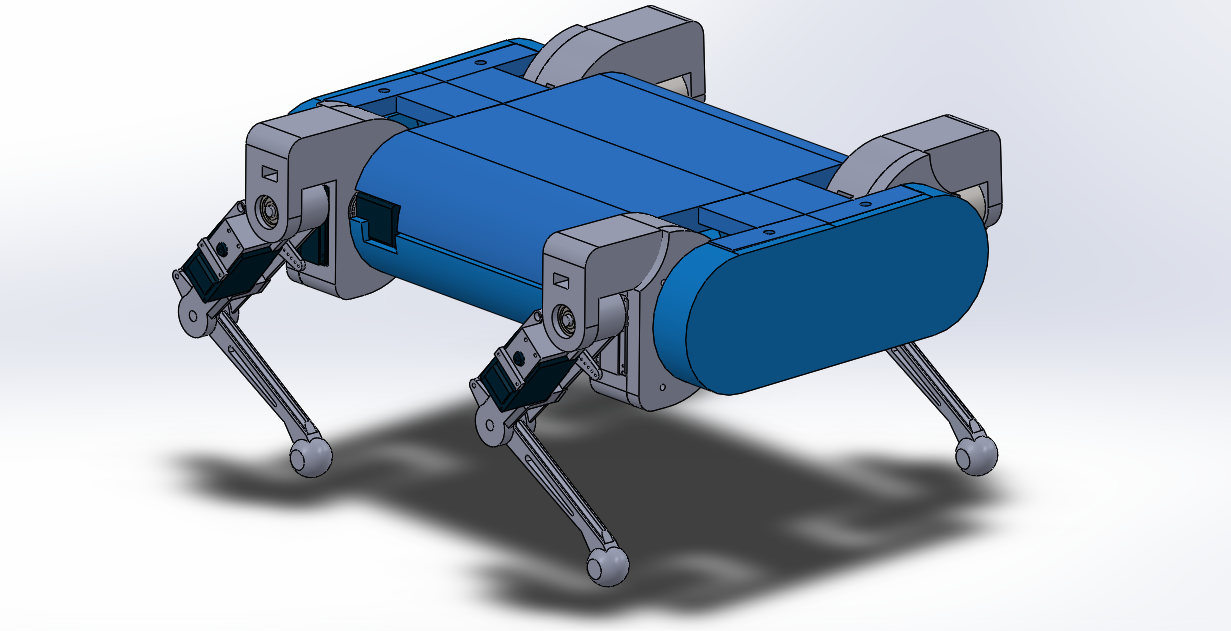
\includegraphics[width=0.6\textwidth]{img/fig19-preview_design.png }
    \caption{3D thiết kế robot Dog}
    \label{fig19}
\end{figure}

\begin{table}[h]
\centering
\caption{Các thông số chính của robot bốn chân}
 \label{tab:2}
\begin{tabular}{ccccccc}
\toprule
Chiều dài & Chiều rộng & Chiều cao & \makecell{Chiều dài\\hông\\$L_1$} & \makecell{Chiều dài\\đùi\\$L_2$} & \makecell{Chiều dài\\cẳng chân\\$L_3$} & \makecell{Bậc\\tự do} \\
\midrule
209 mm & 191 mm & 185 mm & 26 mm & 106 mm & 125 mm & 12 \\
\bottomrule
\end{tabular}
\end{table}

\subsection{Phân tích ngân sách khối lượng}

Việc quản lý khối lượng có ý nghĩa quan trọng đối với robot bốn chân, ảnh hưởng trực tiếp đến mô-men yêu cầu tại các khớp, thời gian hoạt động và tính ổn định. Bảng~\ref{tab:weight_budget} trình bày phân tích chi tiết ngân sách khối lượng của toàn bộ hệ thống.

\begin{table}[H]
\centering
\caption{Ngân sách khối lượng robot bốn chân}
\label{tab:weight_budget}
\renewcommand{\arraystretch}{1.3}
\begin{tabular}{|l|c|c|c|}
\hline
\textbf{Thành phần} & \textbf{Số lượng} & \textbf{Đơn vị (g)} & \textbf{Tổng (g)} \\ \hline
Khung thân (PLA) & 1 & 250 & 250 \\ \hline
Nắp thân (PLA) & 1 & 80 & 80 \\ \hline
Cụm khớp hông (PLA) & 4 & 45 & 180 \\ \hline
Đùi chân (PLA) & 4 & 30 & 120 \\ \hline
Cẳng chân (PLA) & 4 & 25 & 100 \\ \hline
Servo ST3215 & 12 & 69 & 828 \\ \hline
Jetson Nano B01 & 1 & 140 & 140 \\ \hline
IMU BNO055 & 1 & 5 & 5 \\ \hline
Bus Servo Adapter (A) & 2 & 15 & 30 \\ \hline
Mạch giảm áp XL4015 & 1 & 25 & 25 \\ \hline
Ốc vít, ổ bi, phụ kiện & -- & -- & 100 \\ \hline
Cáp và dây nối & -- & -- & 150 \\ \hline
\midrule
\textbf{Tổng cộng} & & & \textbf{$\sim$2008} \\ \hline
\end{tabular}
\end{table}

Kết quả cho thấy khối lượng robot (không bao gồm nguồn và cáp nguồn) vào khoảng 2,0 kg, phù hợp với giá trị $M = 2{,}3$ kg đã sử dụng trong các tính toán mô-men ở các mục trước (bao gồm cả cáp nguồn). Phần lớn khối lượng đến từ 12 servo ($\sim$41\%), tiếp theo là khung thân và phụ kiện PLA ($\sim$36\%).

\subsection{Quy trình lắp ráp}

Quy trình lắp ráp robot bốn chân được thực hiện theo các bước tuần tự sau:

\begin{enumerate}
    \item \textbf{Lắp ráp khớp hông:} Gắn servo hip roll vào giá đỡ khớp hông, lắp ổ bi 626zz ở phía đối diện. Sau đó lắp servo hip pitch bên trong giá đỡ.
    \item \textbf{Lắp ráp chân:} Gắn servo knee (gối) vào phần trên của đùi, nối cẳng chân qua cơ cấu tay đòn và thanh liên kết ball-head.
    \item \textbf{Nối chân với thân:} Lắp 4 cụm khớp hông vào 4 góc của thân robot. Đảm bảo các trục servo hip roll song song với trục dọc thân.
    \item \textbf{Đi dây servo:} Nối cáp tín hiệu từ 12 servo về hai mạch Bus Servo Adapter. Nhóm cáp theo danh tính driver (A: chân LF+RB, B: chân LB+RF).
    \item \textbf{Lắp điện tử:} Gắn Jetson Nano, IMU BNO055, mạch giảm áp XL4015 và hai Bus Servo Adapter vào bên trong thân robot.
    \item \textbf{Kết nối nguồn:} Nối nguồn xung 12V vào hai Bus Servo Adapter (cấp cho servo) và mạch giảm áp (cấp 5V cho Jetson Nano).
    \item \textbf{Kiểm tra:} Cấp nguồn và chạy chương trình calibrate để xác minh chiều quay, ID servo và phạm vi góc quay của từng khớp.
\end{enumerate}

Toàn bộ quá trình lắp ráp từ các chi tiết in 3D đến robot hoàn chỉnh có thể vận hành mất khoảng 4--5 giờ, không bao gồm thời gian in 3D và calibrate phần mềm.